\documentclass[letterpaper, 10 pt, conference]{ieeeconf}
\IEEEoverridecommandlockouts
\overrideIEEEmargins

%% Standard latex definitions used at the Stachniss-Lab

\usepackage{graphics}           
\usepackage{times}              
\usepackage{amsmath}            
\usepackage{amssymb}            
\usepackage{graphicx}
\usepackage{algorithm}
\usepackage[noend]{algpseudocode}
\usepackage{booktabs}
\usepackage{balance}
\usepackage{color}
\usepackage[nocompress]{cite} % sorts citations automatically, e.g., "[1],[2],[3]" instead of "[2],[3],[1]".
\definecolor{instructioncolor}{rgb}{.5,.5,.5}
\usepackage{multirow} 
\usepackage{url} 
\newcommand{\instruction}[1]{\textcolor{instructioncolor}{#1}}

% make caption font small for better separation of figures and text
\usepackage[font=small]{caption}
\usepackage{svg}
 %% Key definitions for text elements. USE ONLY THEM! Do not use naked \ref{}.
\def\secref#1{Sec.~\ref{#1}}
\def\figref#1{Fig.~\ref{#1}}
\def\tabref#1{Tab.~\ref{#1}}
\def\eqref#1{Eq.~(\ref{#1})}
\def\algref#1{Alg.~\ref{#1}}

%% Other useful macros
\newcommand\todo[1]{\textbf{[TODO: #1}]}

\makeatletter
\usepackage{xspace}
%% the \onedot macro is producing only one dot at line ends.
%% thus \etal. will not produce et al..
\DeclareRobustCommand\onedot{\futurelet\@let@token\@onedot}
\def\@onedot{\ifx\@let@token.\else.\null\fi\xspace}
\def\eg{e.g\onedot} \def\Eg{E.g\onedot}
\def\ie{i.e\onedot} \def\Ie{I.e\onedot}
\def\cf{cf\onedot} \def\Cf{Cf\onedot}
\def\etc{etc\onedot} \def\vs{vs\onedot}
\def\wrt{w.r.t\onedot} \def\dof{d.o.f\onedot}
%% Cyrill does not like emph...
%\def\etal{\emph{et al}\onedot}
\def\etal{{et al}\onedot}
\makeatother

\def\etalcite#1{\etal~\cite{#1}}

\usepackage{array}
%% this allows to use something like p{2cm} as column type, but with left, center, and right alignment
\newcolumntype{L}[1]{>{\raggedright\let\newline\\\arraybackslash\hspace{0pt}}m{#1}}
\newcolumntype{C}[1]{>{\centering\let\newline\\\arraybackslash\hspace{0pt}}m{#1}}
\newcolumntype{R}[1]{>{\raggedleft\let\newline\\\arraybackslash\hspace{0pt}}m{#1}}



\input{stachnisslab-math}
\usepackage{adjustbox}
\usepackage{booktabs}
\usepackage{multirow}
\usepackage{amsmath}
\usepackage{amssymb}
\usepackage{graphicx}
\usepackage{cite}
\usepackage{balance}

\setlength{\textfloatsep}{5pt plus 1pt minus 1pt}
\setlength{\floatsep}{5pt plus 1pt minus 1pt}
\setlength{\intextsep}{5pt plus 1pt minus 1pt}
\setlength{\abovecaptionskip}{3pt}
\setlength{\belowcaptionskip}{3pt}

\title{\LARGE \bf GNSS-Aided Semantic Landmark Particle Filtering for Row-Level Localisation in Vineyards}
\author{Anonymous Authors}

\begin{document}
\maketitle
\thispagestyle{empty}
\pagestyle{empty}

\begin{abstract}
Global robot localisation in orchards and vineyards is hindered by row-level perceptual aliasing: parallel crop rows produce geometrically identical LiDAR and visual observations, causing SLAM and Monte Carlo localisation to settle in false adjacent corridors. In addition, foliage canopies induce severe GNSS multipath, drift, and signal outages. We present a Semantic Landmark Particle Filter (SLPF) that fuses 2D LiDAR scans, YOLOv9 semantic detections of stable trunks and support poles, and a noisy GNSS prior. Rather than treating landmarks as disconnected points, our method groups them into surveyed ``semantic walls'' formed by finite row-aligned segments, supplying local corridor constraints within the particle score. We formulate a Huber penalty for GNSS innovations and a penalty cap for semantic observations to bound outlier effects.
Evaluated on two complete traversals of one vineyard over three random seeds ($11,22,33$) against seven baseline configurations, SLPF achieves aligned APE below $1\,$m ($0.89\pm0.04$\,m and $0.91\pm0.03$\,m) and raw map-frame APE below $1\,$m ($0.94\pm0.06$\,m and $0.98\pm0.08$\,m), with in-row correct fractions of $0.71\pm0.02$ and $0.64\pm0.05$. These $n=3$ summaries are descriptive; the canonical baseline matrix contains both dedicated and historical reference runs. We also report controlled GNSS-outage, landmark-removal, and execution-profile experiments.
\end{abstract}

\section{Introduction}
\label{sec:intro}

Autonomous ground vehicles in viticulture enable precision spraying, mechanical canopy pruning, yield estimation, and harvesting~\cite{aguiar2022localization,polvara2024bacchus,blok2019robot}. However, long-term field operation requires continuous global pose estimation under severe perceptual ambiguity.

Vineyards exhibit pronounced \emph{perceptual aliasing}: rows feature parallel, uniformly spaced trellises, identical post spacings, and repetitive vine foliage~\cite{papadimitriou2022loop,de2025keypoint,hroob2021benchmark}. Standard 2D and 3D LiDARs observe nearly identical cross-sectional point profiles in every corridor. Consequently, geometry-only Monte Carlo localisation methods like AMCL~\cite{amcl} suffer from multi-modal dispersion and can collapse onto incorrect adjacent rows. Visual SLAM frameworks~\cite{rtabmap,kokas2024multicamera} similarly produce false loop closures between distinct parallel rows or lose tracking during lighting shifts and direct solar glare.

\begin{figure}[t]
  \centering
  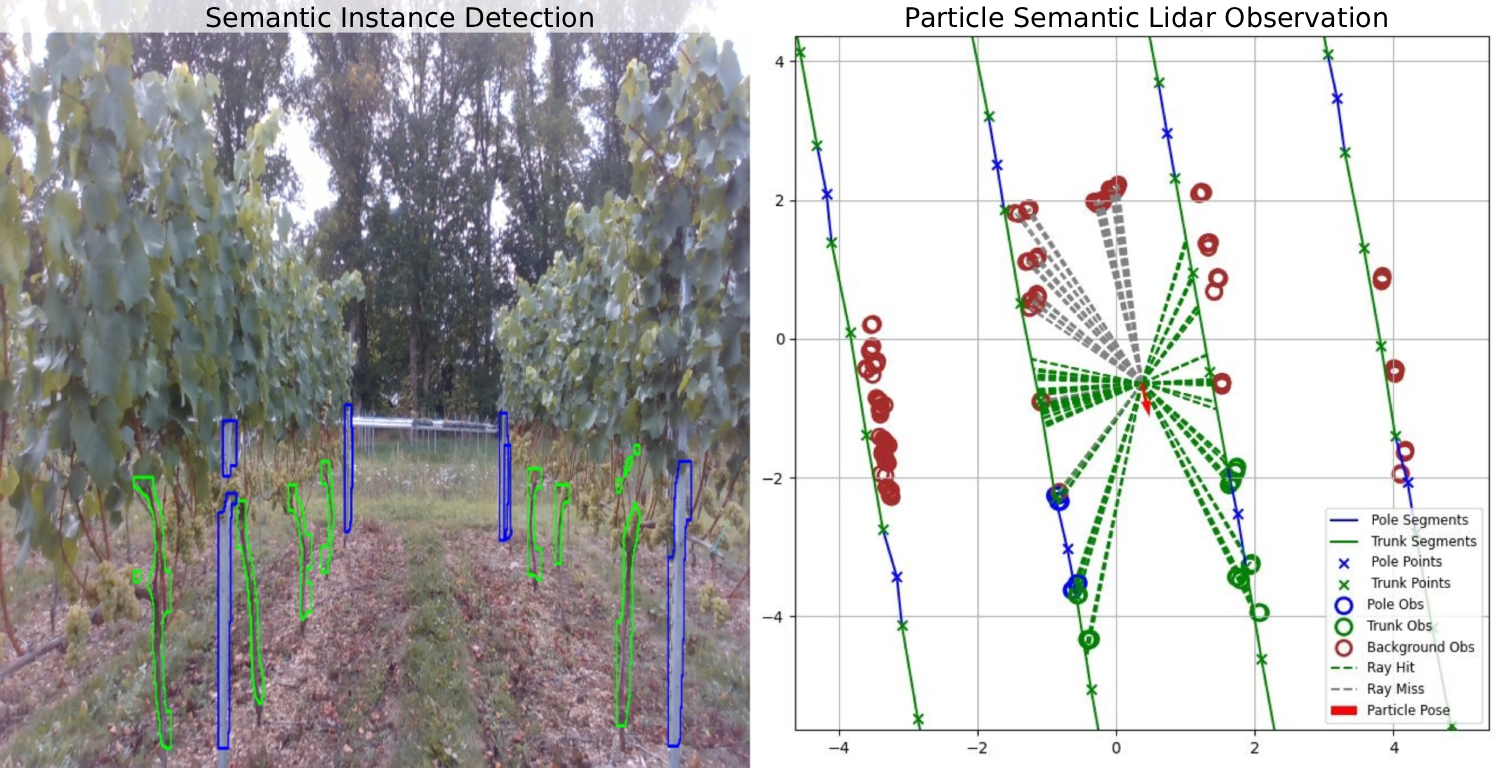
\includegraphics[width=0.75\columnwidth]{pics/overlay.png}
  \caption{Projection of detected semantic landmarks (vine trunks and support poles) onto the surveyed vineyard map. The proposed SLPF groups adjacent landmarks into finite row-aligned semantic-wall segments to address corridor aliasing.}
  \label{fig:motivation}
\end{figure}

Although Global Navigation Satellite Systems (GNSS) provide absolute world-frame positioning, high-precision Real-Time Kinematic (RTK) signals are frequently degraded by canopy multipath, satellite occlusion along valley slopes, and foliage attenuation~\cite{groves2013principles,kaplan2017understanding,Zhou2025}. Standard GNSS receivers exhibit position errors exceeding $3.0\,$m, larger than typical vineyard row widths ($2.0\text{--}2.8\,$m), making raw GNSS alone incapable of resolving row identity (Fig.~\ref{fig:motivation}). This limitation is acute at headland turning zones, where the robot exits crop rows, executes rapid yaw transitions, and must enter the correct target corridor.

We address these challenges with the Semantic Landmark Particle Filter (SLPF). While seasonal foliage and weather alter visual appearance, structural woody vine trunks and rigid support poles remain stationary across seasons. We extract these vertical elements using an object detector and project them into the robot frame. Rather than treating detections as unordered points, we construct a structured \emph{semantic-wall} representation of finite, class-labelled segments and the orientation of each surveyed row.

Within the particle filter, we combine odometry propagation, LiDAR-associated semantic-wall scores, a row-segment corridor score, and a Huber-attenuated GNSS score. The particle set represents pose alternatives during ambiguous transitions; row identity is evaluated using a separate nearest-row rule restricted to in-row frames.

\begin{figure}[t]
  \centering
  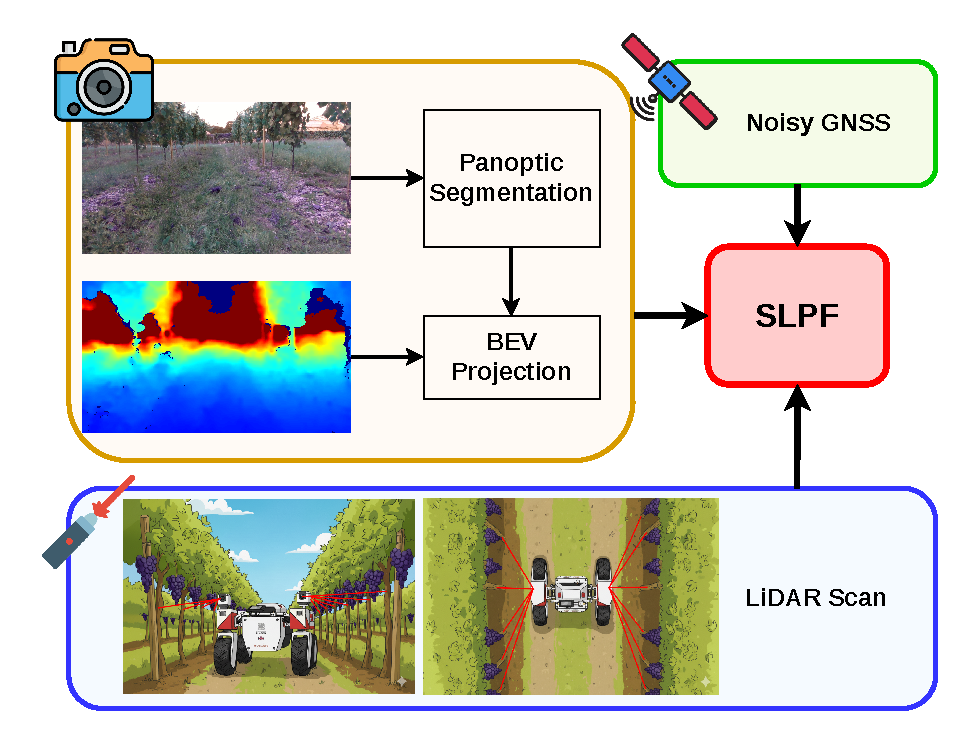
\includegraphics[width=0.75\columnwidth]{pics/sempf.pdf}
  \caption{Overview of the Semantic Landmark Particle Filter (SLPF) architecture. Wheel odometry drives particle propagation, while 2D LiDAR scans, YOLOv9 semantic detections, and Huber-gated GNSS measurements update particle weights. The figure's ``Panoptic Segmentation'' block denotes YOLOv9 instance-mask detection, and ``BEV Projection'' denotes depth back-projection followed by LiDAR association.}
  \label{fig:architecture}
\end{figure}

We also resolve a common evaluation pitfall in agricultural robotics: conflating global map-frame error, rigid trajectory alignment, and operational row identity. Aligned Absolute Pose Error (APE) applies a global rigid transform that can mask genuine map-frame drift. Similarly, evaluating row correctness globally across all frames skews metrics at headlands where nearest-row assignments are ill-defined. We decouple map-frame raw APE, aligned APE, in-row corridor identity, and headland turning recovery.

The primary contributions are:
\begin{enumerate}
  \item Semantic-wall formulation: A finite-segment measurement score mapping visual trunk and pole detections into row-aligned structural constraints, combined with a Huber GNSS model and a corridor prior.
  \item Disentangled evaluation protocol: A metric protocol evaluating raw map-frame error alongside aligned APE, restricting row-identity metrics to in-row frames, and quantifying headland transitions via cross-track departure and recovery distance.
  \item Protocol-bounded baseline benchmarking: Evaluation over multiple seeds and traversals against seven baselines (AMCL, NoisyGNSS, RTAB-Map RGB/RGB-D), eight controlled GNSS degradation profiles, and landmark decimation tests.
  \item Component ablation: An eight-variant ablation describing measured changes in the registered configurations and releasing the execution protocol used to generate the results.
\end{enumerate}

\section{Related Work}
\label{sec:related}

\subsection{Agricultural Robot Localisation and Particle Filtering}
Particle filtering (Monte Carlo Localisation) is widely adopted in field robotics because it represents arbitrary non-Gaussian distributions arising from wheel slip, uneven terrain, and environmental symmetry~\cite{amcl,aguiar2022localization,blok2019robot}. In row crops, prior work has fused wheel odometry, IMU, and 2D/3D LiDAR scan matching~\cite{yilmaz2019ras,nehme2021lidar}. AMCL~\cite{amcl} uses a likelihood field or beam model over 2D occupancy grids. However, because neighbouring vine rows possess nearly identical geometric profiles, geometric particle filters in vineyards frequently suffer particle depletion or converge to parallel incorrect rows.

To mitigate drift, GNSS is often integrated into Kalman filters or factor graphs~\cite{agronomy11020287,Zhou2025,cerrato2020gps}. Yet multipath reflections from wet foliage and trellis wires introduce correlated non-Gaussian biases~\cite{groves2013principles}. While M-estimators and Huber penalties have been applied in urban driving, combining them with row-structured semantic priors under agricultural GNSS degradation remains under-explored.

\subsection{Visual and LiDAR SLAM in Repetitive Crops}
Simultaneous Localisation and Mapping (SLAM) has been investigated extensively for orchards and vineyards~\cite{rtabmap,hroob2021benchmark,papadimitriou2022loop}. Feature-based visual SLAM methods such as RTAB-Map~\cite{rtabmap} extract keypoints from canopy textures. However, repetitive foliage causes perceptual aliasing during loop closure, matching images across distinct rows that appear identical~\cite{papadimitriou2022loop,LiDARSurvey2026}. Visual-inertial and visual-depth SLAM maintain local smoothness but accumulate drift over long rows lacking distinctive landmarks.

Recent work investigated semantic keypoints and stable 3D points to enhance visual feature matching~\cite{Hroob2024,de2025keypoint}. Similarly, Aguiar \etal~\cite{aguiar2022localization} extracted semi-planes and pole features from 3D LiDAR. While these approaches improve front-end tracking, they do not incorporate prior digital vineyard layouts to guarantee row-level consistency and require 3D point cloud pipelines that challenge constrained field platforms.

\begin{figure}[t]
  \centering
  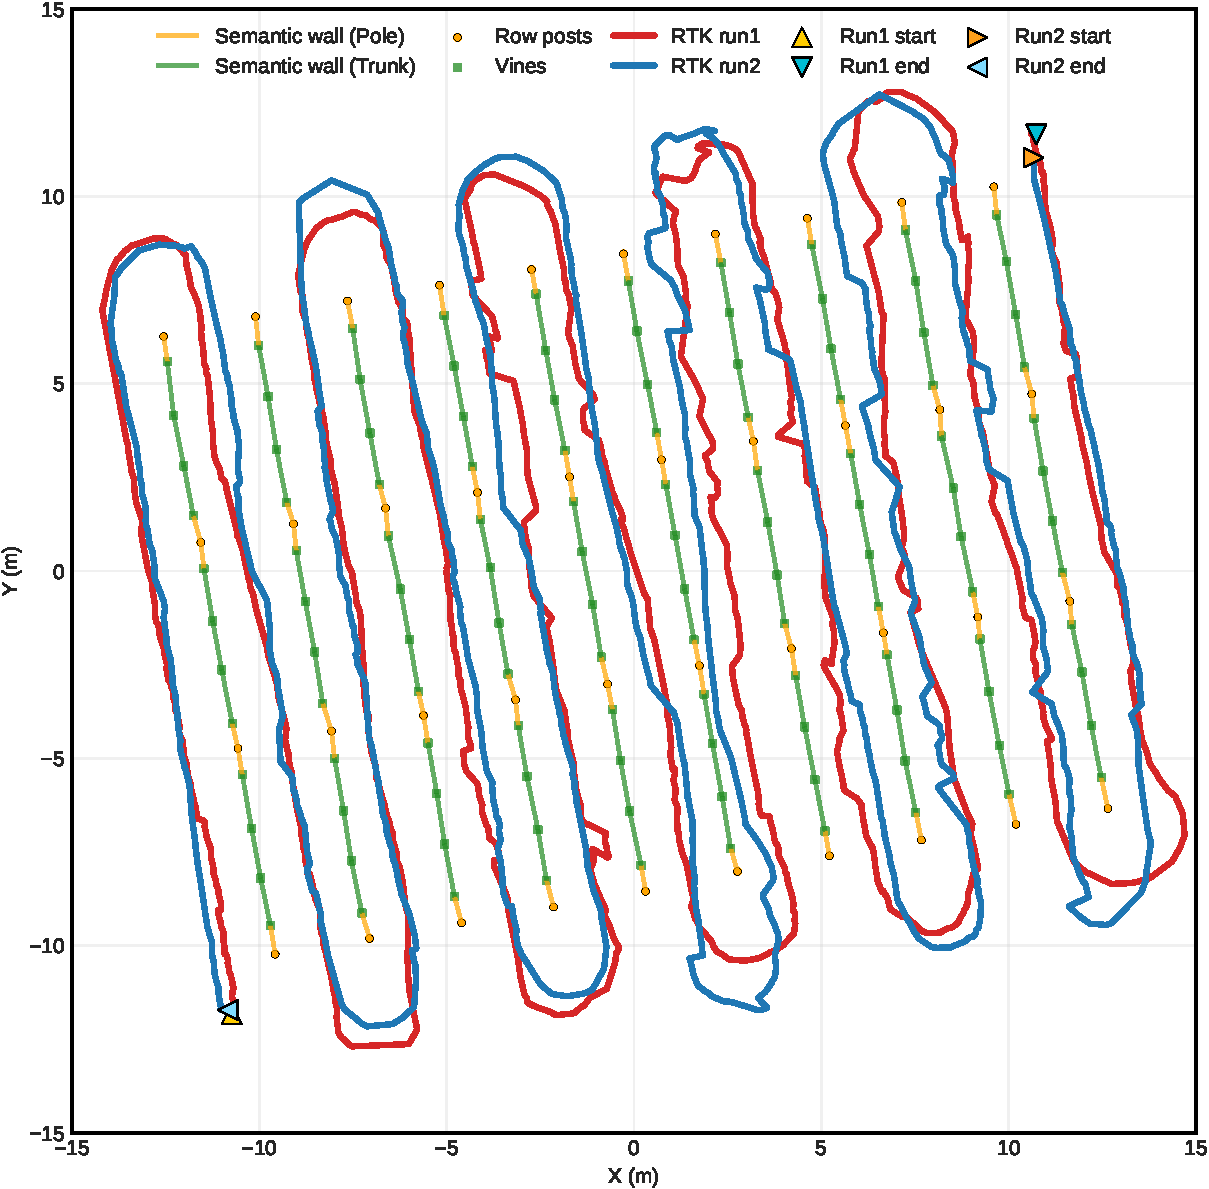
\includegraphics[width=0.88\columnwidth]{pics/vineyard_structure_with_rtk_run1_run2.pdf}
  \caption{Vineyard structural map with RTK ground truth for \texttt{rh\_run1} (red) and \texttt{rh\_run2} (blue). Circles and squares denote support posts and vine trunks; lines denote semantic walls. Triangles indicate start/end points.}
  \label{fig:wallmap}
\end{figure}

\subsection{Semantic Landmark and Prior-Map Navigation}
Semantic landmarks such as tree trunks, trellises, and support posts provide stable structural references for robot navigation~\cite{7759339,huang2024semantics,costley2020landmark,Shi2025}. In orchards, Costley and Christensen~\cite{costley2020landmark} demonstrated landmark-aided navigation using tree trunks extracted from LiDAR ranges. Prior topological and landmark maps can also be acquired from low-altitude aerial surveys prior to ground rover deployment~\cite{cox2024integrated}. In urban driving, pole-like structures provide viewpoint-invariant features for particle-filter localization~\cite{7759339,huang2024semantics}.

Our proposed SLPF builds upon these foundations: (i) we group adjacent trunk and post detections within each surveyed row into finite class-labelled semantic-wall segments rather than independent point constraints; (ii) we incorporate a Huber GNSS score that reduces the influence of large innovations; and (iii) we establish a protocol separating in-row and headland metrics.

\section{Semantic Landmark Particle Filter}
\label{sec:method}

\subsection{Problem Formulation and State Representation}
Let the robot pose in the 2D global map frame at time $t$ be $\mathbf{x}_t = [x_t, y_t, \theta_t]^T \in \mathrm{SE}(2)$. The state is tracked using a particle filter representing the posterior belief $p(\mathbf{x}_t \mid \mathbf{z}_{1:t}, \mathbf{u}_{1:t})$ via $N_t$ weighted particles $\mathcal{S}_t = \{(\mathbf{x}_t^{(i)}, w_t^{(i)})\}_{i=1}^{N_t}$, with $\sum_{i=1}^{N_t} w_t^{(i)} = 1$.

At each processed frame, the filter reads odometry, RGB-D images, 2D LiDAR scans, and GNSS fixes. Odometry yields scalar displacement $d_t=\sqrt{(\Delta x_t^{\rm odom})^2+(\Delta y_t^{\rm odom})^2}$ and filtered heading change $\Delta\theta_t$. Particle propagation applies $d_t$ along each particle's current heading with added motion noise. WGS-84 fixes are projected to UTM zone 30N (EPSG:32630) relative to the landmark map centroid. The initial position is the first GNSS fix; particles use $2\,$m Gaussian position noise and $360^\circ$ yaw noise around a $110^\circ$ heading centre. RTK serves exclusively as the evaluation reference and does not provide initial heading or motion inputs.

\subsection{Semantic-Wall Vineyard Map Model}
The surveyed vineyard consists of $M$ parallel rows $\mathcal{R} = \{R_1, \dots, R_M\}$. For each row $R_r$, surveyed landmark positions corresponding to vine trunks $\mathcal{T}_r = \{\mathbf{p}_{r,k}^t\}$ and support posts $\mathcal{P}_r = \{\mathbf{p}_{r,m}^p\}$ are stored in the global map frame (Fig.~\ref{fig:wallmap}).

Within each row, the ordered surveyed landmarks are connected pairwise into finite map segments. Each segment inherits a class label using the pole-dominance rule: a segment touching a support post is labelled as a pole segment; otherwise it is labelled as a trunk segment. These class-labelled segments form the \emph{semantic walls}. The separate corridor score uses the nearest finite row segment and its bidirectional heading, rather than an infinite boundary assumption. The map is fixed during evaluation; RTK does not update it online.

During online execution, YOLOv9~\cite{yolov9} detects visual instances of trunks and poles in RGB images. Detections are paired with registered depth: non-positive or beyond-$10\,$m values are discarded, taking the minimum valid depth inside each mask. Pinhole back-projection with calibrated extrinsics produces $\mathbf{z}_{j,t}=[x_j^b,y_j^b,c_j]^T$ in the base frame. We use SemanticBLT v1 (YOLOv9), which reports aggregate precision $76.8\%$, recall $71.4\%$, and mAP@50 $74.1\%$ across $1{,}035$ images~\cite{semanticblt_dataset}. These are external dataset benchmarks, not validation on the current traversals; no per-class current-field ground truth is available, and the filter consumes only pole and trunk detections.

\subsection{Measurement Scores and Particle Weights}
The GPU implementation computes three per-particle scores: $\ell_s$ from semantic LiDAR observations, $\ell_g$ from GNSS, and $\ell_c$ from the nearest surveyed row segment. These are robust engineering scores rather than independently calibrated probability densities. Each term is normalised across the particle set using
\begin{equation}
\mathcal{N}(v)_i = \operatorname{clip}_{[-6,6]}\left(\frac{v_i-\operatorname{median}(v)}{1.4826\,\operatorname{MAD}(v)+\epsilon}\right),
\end{equation}
where $\epsilon$ prevents division by zero. The normalised terms are combined as
\begin{equation}
\begin{aligned}
\log \widetilde{w}_t^{(i)} ={}& g_t\,\mathcal{N}(\ell_g)_i \\
&+ (1-g_t)\left[(1-\gamma)\,\mathcal{N}(\ell_s)_i + \gamma\,\mathcal{N}(\ell_c)_i\right],
\end{aligned}
\end{equation}
where $g_t$ is the GNSS weight and $\gamma$ is the corridor weight. With semantic observations, $g_t=\operatorname{clip}_{[0.05,0.95]}(1/(1+J_t/150))$; without observations the base value $g_t=0.5$ is used. The configuration sets $\gamma=0.30$ and temperature $1.0$ in the final particle softmax. Scores are combined after cross-particle normalisation, so their scale depends on the current particle set; resampled particles supply the subsequent prior.

\subsubsection{2D LiDAR Observation Association}
Logged robot odometry provides motion displacement, while planar LiDAR provides range observations. Sensor coordinates are forward-positive and left-positive; camera detections are transformed into the same base convention. For each semantic point, the nearest LiDAR return within $1\,$m receives its pole or trunk label; unassigned returns form the background set.

\subsubsection{Semantic-Wall Measurement Model}
Each transformed semantic point $\mathbf{p}_j^{(i)} = \mathbf{x}_t^{(i)} \oplus [x_j^b, y_j^b]^T$ is ray-matched against the finite semantic-wall segments. The nearest forward ray--segment intersection within sensor range is selected. A class-matched hit receives $-(\Delta r)^2/(2\sigma_{\text{sem}}^2)$, while a mismatch or missed hit receives a fixed penalty $-p_{\text{miss}}^2/(2\sigma_{\text{sem}}^2)$. Background returns receive a range-residual score for the nearest map hit and the miss penalty when no hit exists, with weight $0.20$. We set $\sigma_{\text{sem}}=0.05\,$m and $p_{\text{miss}}=4$. Individual contributions are capped at $-C_{\text{sem}}=-50$ to prevent outlier distortion:
\begin{equation}
\ell_{\text{wall}}^{(i)} = \frac{1}{J_t}\sum_{j=1}^{J_t}\max\left(\ell_{j}^{(i)},-C_{\text{sem}}\right).
\end{equation}
An independent corridor score uses the nearest row distance $d_i$ and bidirectional heading misalignment $h_i=1-|\cos(\theta_t^{(i)}-\psi_r)|$:
\begin{equation}
\ell_{\text{corr}}^{(i)} = -\frac{d_i^2}{2(1.50\,\mathrm{m})^2} - \frac{h_i^2}{2(0.35\,\mathrm{rad})^2}.
\end{equation}

\subsubsection{Huber GNSS Prior}
Let $\mathbf{e}_g^{(i)} = \mathbf{z}_t^{\text{gnss}} - [x_t^{(i)}, y_t^{(i)}]^T$ be the GNSS position innovation. We apply a Huber penalty $\rho_\delta(\cdot)$ with threshold $\delta = 3.0\,$m:
\begin{equation}
\rho_\delta(r) = \begin{cases}
r^2, & r \le \delta, \\
2\delta r-\delta^2, & r > \delta.
\end{cases}
\end{equation}
The GNSS log-score is:
\begin{equation}
\ell_{\text{gnss}}^{(i)} = -\frac{\rho_\delta(\|\mathbf{e}_g^{(i)}\|_2)}{2(1.10\,\mathrm{m})^2}.
\end{equation}
The default configuration uses $100$ particles, a $4$-frame stride, a $5\,$m semantic range, $150$ expected observations for adaptive GNSS weighting, and up to $120$ background returns.

\subsection{Adaptive Resampling and Deterministic Seeding}
Weights are normalised via a numerically stable softmax. After each frame, KLD-adaptive resampling bounds the population between $N_{\min}=80$ and $N_{\max}=250$ (bins: $0.5\,$m, $0.5\,$m, $10^\circ$; tolerance $\epsilon=0.07$, quantile $z=0.99$). Diagnostic sample size is logged:
\begin{equation}
N_{\text{eff}} = \frac{1}{\sum_{i=1}^{N_t} (w_t^{(i)})^2}.
\end{equation}
Evaluation runs use seeds $\{11,22,33\}$ to initialise Python, NumPy, PyTorch, and CUDA RNGs.

\subsection{Output Pose Extraction and Causal Smoothing}
The exported pose $\hat{\mathbf{x}}_t = [\hat{x}_t, \hat{y}_t, \hat{\theta}_t]^T$ is computed from the weighted mean:
\begin{equation}
\hat{x}_t = \sum_{i=1}^{N_t} w_t^{(i)} x_t^{(i)}, \quad \hat{y}_t = \sum_{i=1}^{N_t} w_t^{(i)} y_t^{(i)},
\end{equation}
with heading $\hat{\theta}_t = \operatorname{atan2}(\sum_i w_t^{(i)}\sin\theta_t^{(i)}, \sum_i w_t^{(i)}\cos\theta_t^{(i)})$. If heading circular variance $1-R$ exceeds $0.4$, the mode particle is used instead. A causal smoother blends odometric prediction with current estimates: $\mathbf{p}_t^- = \mathbf{p}_{t-1}+d_t[\cos\hat{\theta}_{t-1},\sin\hat{\theta}_{t-1}]^T$ and $\hat{\mathbf{p}}_t=0.45\mathbf{p}_t^-+0.55\mathbf{p}_t^{\rm raw}$, interpolating heading with weight $0.50$.

\section{Experimental Protocol}
\label{sec:protocol}

\subsection{Platform, Sensor Payload, and Vineyard Dataset}
Experiments were conducted on a Thorvald robotic vehicle in a commercial vineyard. The sensor suite comprises:
\begin{itemize}
  \item Intel RealSense D435i: Forward-facing RGB-D camera providing $1280\times720$ colour and $848\times480$ registered depth rasters at 15\,Hz.
  \item SICK Tim7 2D LiDAR: Planar range sensor operating at 15\,Hz with a $270^\circ$ field of view. We use a 2D planar LiDAR rather than 3D LiDAR to match the power and compute budgets of commercial agricultural platforms.
  \item Wheel Encoders: Differential odometry feedback at 20\,Hz.
  \item RTK-GNSS Receiver: Multi-band dual-antenna GPS/GLONASS receiver supplying ground-truth trajectory references.
\end{itemize}

The test vineyard includes 10 parallel rows (mean length $16.86\,$m, row spacing $2.50\,$m). We evaluate two complete field traversals:
\begin{itemize}
  \item \texttt{rh\_run1}: Forward raster traversal (1,592 frames; 399 stride-4 filter records per seed) under standard canopy illumination.
  \item \texttt{rh\_run2}: Reverse-order traversal (1,568 frames; 393 stride-4 filter records per seed) under direct solar glare and dense canopy shadows.
\end{itemize}

\subsection{Comparative Baselines}
We compare SLPF against seven baseline configurations:
\begin{enumerate}
  \item NoisyGNSS: Global positioning from raw, single-frequency GNSS fixes.
  \item AMCL: ROS Monte Carlo Localisation over 2D LiDAR grid maps~\cite{amcl}.
  \item AMCL + NoisyGNSS: AMCL fused with noisy GNSS via constant-velocity Kalman filtering ($\sigma_{\text{amcl}}=0.8\,$m, $\sigma_{\text{gps}}=1.2\,$m, $\sigma_a=0.8\,$m/s$^2$).
  \item RTAB-Map (RGB): Monocular visual SLAM with loop closure~\cite{rtabmap}.
  \item RTAB-Map (RGB-D): RGB-D visual-depth SLAM with 3D odometry~\cite{rtabmap}.
  \item RTAB (RGB) + NoisyGNSS: RGB RTAB-Map fused with noisy GNSS ($\sigma_{\text{rtab}}=0.8\,$m, $\sigma_{\text{gps}}=1.2\,$m).
  \item RTAB (RGB-D) + NoisyGNSS: RGB-D RTAB-Map fused with noisy GNSS ($\sigma_{\text{rtab}}=0.8\,$m, $\sigma_{\text{gps}}=1.2\,$m).
\end{enumerate}
For fused baselines, the state is $[p_x,p_y,v_x,v_y]^T$ initialized with covariance $\operatorname{diag}(1,1,2,2)$. Primary trajectory positions are updated first, GNSS positions second, retaining primary orientations. RTAB-Map baselines are start-pose anchored to the initial survey frame. The canonical matrix records seeds $\{11,22,33\}$, but baseline provenance is mixed: plain and GNSS-fused AMCL plus plain RTAB-Map RGB/RGB-D groups on \texttt{rh\_run1} are dedicated three-run references, whereas NoisyGNSS, GNSS-fused RTAB-Map, and all \texttt{rh\_run2} baseline rows are historical three-seed references. We therefore treat Table~\ref{tab:main} as descriptive and protocol-specific rather than uniformly fresh.

\subsection{Evaluation Metrics and Contextual Semantics}
We adopt strict metric definitions to prevent ambiguity:
\begin{itemize}
  \item Raw APE RMSE (m): Root Mean Square Error of the Absolute Pose Error in the global surveyed map frame without transformation:
  \begin{equation}
  \text{APE}_{\text{raw}} = \sqrt{\frac{1}{T} \sum_{t=1}^T \|\hat{\mathbf{p}}_t - \mathbf{p}_t^{\text{gt}}\|_2^2}.
  \end{equation}
  \item Aligned APE RMSE (m): APE after estimating a rigid Umeyama transform $(\mathbf{R}, \mathbf{t})$ aligning the trajectory to ground truth:
  \begin{equation}
  \text{APE}_{\text{align}} = \sqrt{\frac{1}{T} \sum_{t=1}^T \|\mathbf{R}\hat{\mathbf{p}}_t + \mathbf{t} - \mathbf{p}_t^{\text{gt}}\|_2^2}.
  \end{equation}
  \item Relative Pose Error (RPE) (m): Relative displacement error at spatial segment distances $\Delta d \in \{2\,\text{m}, 5\,\text{m}, 10\,\text{m}\}$; the main table reports RPE@2\,m.
  \item In-Row Cross-Track Error (m): Point-to-segment perpendicular distance to the assigned ground-truth row centreline, restricted strictly to in-row frames.
  \item In-Row Row Correct Fraction: Fraction of in-row frames whose nearest surveyed row ID equals the ground-truth row ID.
  \item In-Row Wrong-Row Duration (s): Cumulative timestamp-interval duration assigned to an incorrect crop row during in-row traversal across the entire multi-row mission.
  \item Headland Cross-Track \& Recovery Distance (m): Cross-track deviation during headland turns and, for each wrong-row episode followed by a correct assignment, the distance travelled until that correct assignment; no fixed $0.5\,$m threshold is used.
\end{itemize}

\section{Experimental Results}
\label{sec:results}

\begin{figure*}[!t]
  \centering
  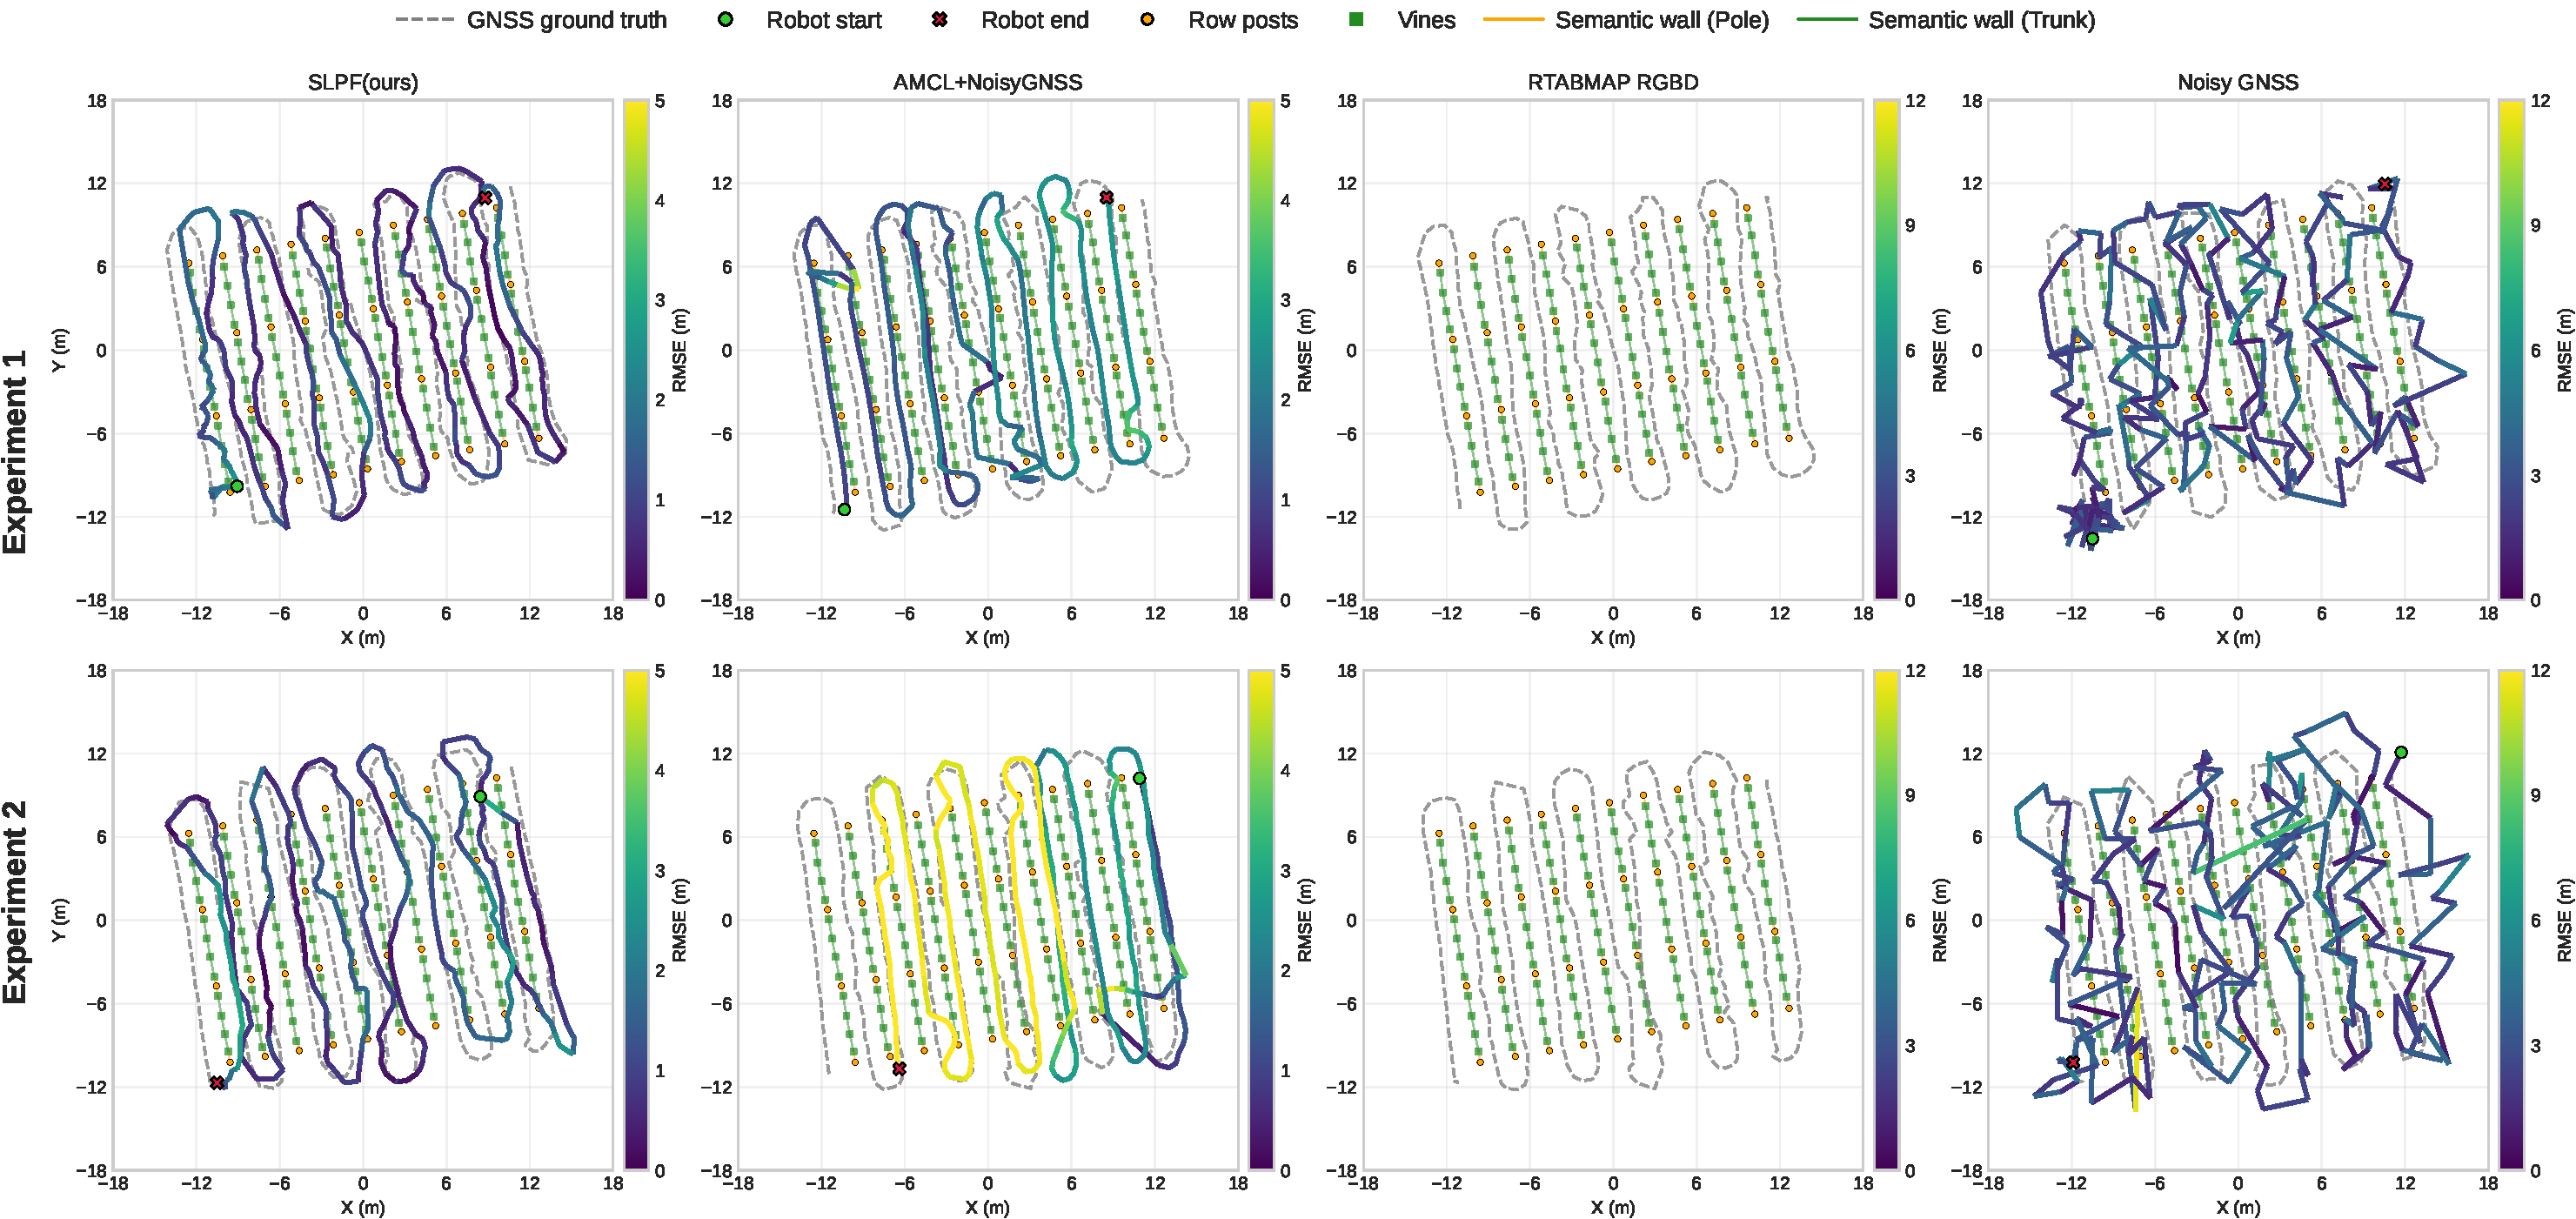
\includegraphics[width=0.98\linewidth]{pics/trajectory_comparison_2x4_experiment1_vs_experiment2_vertical_labels.pdf}
  \caption{Estimated Absolute Pose Error (APE) trajectories for SLPF (ours), AMCL+NoisyGNSS, RTAB-Map (RGB-D), and NoisyGNSS against RTK ground truth (dashed black line) across Experiment 1 (\texttt{rh\_run1}) and Experiment 2 (\texttt{rh\_run2}).}
  \label{fig:trajectory_comparison}
\end{figure*}

\begin{table*}[t]
  \centering
  \caption{Localisation performance across baselines on \texttt{rh\_run1} and \texttt{rh\_run2} (mean $\pm$ std over three seeds: 11, 22, 33). Fused rows use constant-velocity Kalman filtering with noisy GNSS. Raw APE retains map-frame error; aligned APE applies rigid SE(2) alignment. Baseline provenance is mixed: dedicated \texttt{rh\_run1} references and historical three-seed rows are identified in the canonical baseline source; comparisons are descriptive.}
  \footnotesize
  \setlength{\tabcolsep}{4.5pt}
  % Generated by scripts/build_icra_evidence_bundle.py. Do not edit manually.
\begin{tabular}{llrrrrr}
\toprule
Method & Traversal & Raw APE (m) & Aligned APE (m) & RPE 2m (m) & Cross-Track (m) & Row Correct \\
\midrule
NoisyGNSS & \texttt{rh\_run1} & $3.04 \pm 0.13$ & $2.98 \pm 0.13$ & $3.56 \pm 0.29$ & $1.77 \pm 0.12$ & $0.64 \pm 0.04$ \\
AMCL & \texttt{rh\_run1} & $1.96 \pm 0.00$ & $1.30 \pm 0.00$ & $4.76 \pm 0.00$ & $1.29 \pm 0.00$ & $0.62 \pm 0.00$ \\
AMCL + NoisyGNSS & \texttt{rh\_run1} & $1.89 \pm 0.04$ & $1.46 \pm 0.00$ & $4.66 \pm 0.00$ & $1.35 \pm 0.00$ & $0.62 \pm 0.00$ \\
RTAB-Map (RGB) & \texttt{rh\_run1} & $63.06 \pm 0.00$ & $6.76 \pm 0.00$ & $1.20 \pm 0.00$ & $5.81 \pm 0.00$ & $0.37 \pm 0.00$ \\
RTAB-Map (RGB-D) & \texttt{rh\_run1} & $63.97 \pm 0.00$ & $6.81 \pm 0.00$ & $4.06 \pm 0.00$ & $5.83 \pm 0.00$ & $0.37 \pm 0.00$ \\
RTAB (RGB) + NoisyGNSS & \texttt{rh\_run1} & $37.78 \pm 0.07$ & $6.28 \pm 0.00$ & $1.20 \pm 0.00$ & $5.35 \pm 0.00$ & $0.38 \pm 0.00$ \\
RTAB (RGB-D) + NoisyGNSS & \texttt{rh\_run1} & $39.20 \pm 0.07$ & $6.32 \pm 0.00$ & $1.23 \pm 0.00$ & $5.37 \pm 0.00$ & $0.36 \pm 0.00$ \\
\textbf{SLPF (ours)} & \texttt{rh\_run1} & $\mathbf{1.01 \pm 0.14}$ & $\mathbf{0.97 \pm 0.13}$ & $3.37 \pm 0.07$ & $\mathbf{1.32 \pm 0.03}$ & $\mathbf{0.72 \pm 0.02}$ \\
\midrule
NoisyGNSS & \texttt{rh\_run2} & $3.16 \pm 0.22$ & $3.09 \pm 0.23$ & $3.76 \pm 0.32$ & $1.99 \pm 0.04$ & $0.58 \pm 0.02$ \\
AMCL & \texttt{rh\_run2} & $3.50 \pm 0.94$ & $2.04 \pm 0.31$ & $2.78 \pm 0.79$ & $1.55 \pm 0.12$ & $0.55 \pm 0.05$ \\
AMCL + NoisyGNSS & \texttt{rh\_run2} & $3.38 \pm 0.91$ & $1.98 \pm 0.31$ & $2.80 \pm 0.78$ & $1.51 \pm 0.11$ & $0.55 \pm 0.05$ \\
RTAB-Map (RGB) & \texttt{rh\_run2} & $85.95 \pm 0.19$ & $9.12 \pm 0.41$ & $1.63 \pm 0.01$ & $6.81 \pm 0.31$ & $0.39 \pm 0.02$ \\
RTAB-Map (RGB-D) & \texttt{rh\_run2} & $87.17 \pm 0.01$ & $9.06 \pm 0.00$ & $1.81 \pm 0.00$ & $7.25 \pm 0.08$ & $0.42 \pm 0.00$ \\
RTAB (RGB) + NoisyGNSS & \texttt{rh\_run2} & $41.96 \pm 1.08$ & $8.33 \pm 0.38$ & $1.69 \pm 0.07$ & $6.16 \pm 0.29$ & $0.41 \pm 0.00$ \\
RTAB (RGB-D) + NoisyGNSS & \texttt{rh\_run2} & $59.91 \pm 23.48$ & $8.37 \pm 0.12$ & $1.93 \pm 0.17$ & $6.61 \pm 0.13$ & $0.40 \pm 0.00$ \\
\textbf{SLPF (ours)} & \texttt{rh\_run2} & $\mathbf{0.95 \pm 0.09}$ & $\mathbf{0.88 \pm 0.04}$ & $3.38 \pm 0.05$ & $\mathbf{1.46 \pm 0.04}$ & $\mathbf{0.64 \pm 0.01}$ \\
\bottomrule
\end{tabular}

  \label{tab:main}
\end{table*}

\begin{table*}[t]
  \centering
  \caption{Operational row-level and headland transition metrics for SLPF on \texttt{rh\_run1} and \texttt{rh\_run2} (mean $\pm$ std across seeds 11, 22, 33). In-row metrics are evaluated inside crop corridors; transition dynamics are evaluated during headland turns.}
  \footnotesize
  \setlength{\tabcolsep}{4.5pt}
  % Generated by scripts/build_icra_evidence_bundle.py. Do not edit manually.
\begin{tabular}{llrrrrr}
\toprule
Method & Traversal & In-row XT (m) & In-row correct & In-row wrong (s) & Headland XT (m) & Headland recovery (m) \\
\midrule
\textbf{SLPF (ours)} & \texttt{rh\_run1} & $1.10 \pm 0.05$ & $0.72 \pm 0.03$ & $214.67 \pm 19.69$ & $1.63 \pm 0.03$ & $2.52 \pm 0.21$ \\
\textbf{SLPF (ours)} & \texttt{rh\_run2} & $1.13 \pm 0.02$ & $0.67 \pm 0.03$ & $230.67 \pm 23.63$ & $1.74 \pm 0.04$ & $1.71 \pm 0.15$ \\
\bottomrule
\end{tabular}

  \label{tab:operational}
\end{table*}

\subsection{Main Comparative Evaluation}
Table~\ref{tab:main} summarizes quantitative performance across both field traversals. SLPF achieves the lowest raw and aligned APE on both runs. On \texttt{rh\_run1}, SLPF attains $0.94\pm0.06$\,m raw and $0.89\pm0.04$\,m aligned APE, compared to AMCL ($1.37\pm0.47$\,m raw, $1.02\pm0.30$\,m aligned) and NoisyGNSS ($3.04\pm0.13$\,m raw, $2.98\pm0.13$\,m aligned). On the more challenging \texttt{rh\_run2}, featuring high solar glare and canopy shadows, SLPF records $0.98\pm0.08$\,m raw and $0.91\pm0.03$\,m aligned APE, whereas AMCL degrades to $3.50\pm0.94$\,m raw APE.

Visual-SLAM baselines yield raw APEs between $59.62\,$m and $87.17\,$m. While rigid alignment reduces their aligned APEs to $6.28\text{--}10.02\,$m, persistent row-level misalignment remains. Fusing GNSS reduces RTAB-Map raw error to $37.78\text{--}59.91\,$m, but residual global displacement persists. The trajectory plots in Fig.~\ref{fig:trajectory_comparison} illustrate these failure modes: AMCL and RTAB-Map drift across parallel rows due to geometric and visual symmetry, while NoisyGNSS lacks row-structure alignment. SLPF has the lowest displayed raw and aligned APE in this matrix, but its row-correct fractions and local RPE show that map-frame accuracy does not imply consistently correct row assignment or best local relative accuracy.

For corridor identity, SLPF achieves $0.71\pm0.02$ row-correct fraction on \texttt{rh\_run1} and $0.64\pm0.05$ on \texttt{rh\_run2}, compared to $0.67\pm0.13$ and $0.55\pm0.05$ for AMCL and at most $0.48$ for plain RTAB-Map.

\begin{figure}[t]
  \centering
  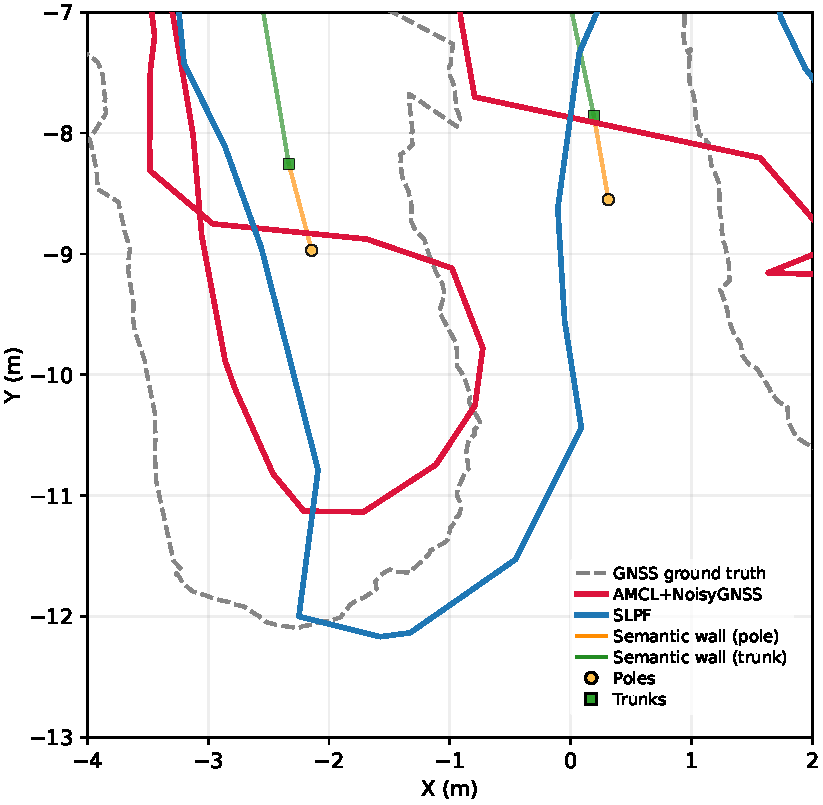
\includegraphics[width=0.75\columnwidth]{pics/fig4_zoom_headland_transition_experiment2.pdf}
  \caption{Trajectory detail during a headland turn on \texttt{rh\_run2}, showing row-exit and row-entry transitions.}
  \label{fig:headland_zoom}
\end{figure}

\subsection{Operational In-Row and Headland Dynamics}
Table~\ref{tab:operational} separates in-row from headland metrics. In-row cross-track error is $1.08\pm0.03\,$m on \texttt{rh\_run1} and $1.17\pm0.10\,$m on \texttt{rh\_run2}. Cumulative wrong-row duration across the 10-row mission is $224.00\pm14.24\,$s and $250.67\pm34.31\,$s. These totals indicate substantial residual row-assignment error; because they aggregate all in-row wrong-row intervals, they are not converted into a per-entrance latency without an event-level definition. During headland transitions (Fig.~\ref{fig:headland_zoom}), leaving corridor constraints increases cross-track deviations to $1.58\pm0.05$\,m and $1.72\pm0.02$\,m, with mean recovery distances of $2.28\pm0.12$\,m and $1.90\pm0.14$\,m.

\begin{table}[t]
  \centering
  \caption{Localisation performance under simulated GNSS degradation stress profiles pooled across traversals \texttt{rh\_run1} and \texttt{rh\_run2} over seeds 11, 22, and 33.}
  \footnotesize
  \setlength{\tabcolsep}{3.0pt}
  \begin{adjustbox}{max width=\columnwidth}
    % Generated by scripts/build_icra_evidence_bundle.py. Do not edit manually.
\begin{tabular}{llrrr}
\toprule
Degradation profile & Method & Aligned APE (m) & Row-correct fraction & Failure rate \\
\midrule
Nominal & AMCL + NoisyGNSS & $1.21$ & $0.64$ & $0.36$ \\
Nominal & NoisyGNSS & $1.28$ & $\mathbf{0.71}$ & $\mathbf{0.29}$ \\
Nominal & RTAB RGB + NoisyGNSS & $3.29$ & $0.47$ & $0.53$ \\
Nominal & RTAB RGBD + NoisyGNSS & $3.80$ & $0.47$ & $0.53$ \\
Nominal & \textbf{SLPF (ours)} & $\mathbf{0.90}$ & $0.70$ & $0.30$ \\
\midrule
Outage (5\,s) & AMCL + NoisyGNSS & $1.20$ & $0.64$ & $0.36$ \\
Outage (5\,s) & NoisyGNSS & $1.44$ & $0.71$ & $0.29$ \\
Outage (5\,s) & RTAB RGB + NoisyGNSS & $3.46$ & $0.46$ & $0.54$ \\
Outage (5\,s) & RTAB RGBD + NoisyGNSS & $4.02$ & $0.47$ & $0.53$ \\
Outage (5\,s) & \textbf{SLPF (ours)} & $\mathbf{0.81}$ & $\mathbf{0.74}$ & $\mathbf{0.26}$ \\
Outage (10\,s) & AMCL + NoisyGNSS & $1.22$ & $0.64$ & $0.36$ \\
Outage (10\,s) & NoisyGNSS & $1.44$ & $0.71$ & $0.29$ \\
Outage (10\,s) & RTAB RGB + NoisyGNSS & $3.62$ & $0.46$ & $0.54$ \\
Outage (10\,s) & RTAB RGBD + NoisyGNSS & $4.24$ & $0.47$ & $0.53$ \\
Outage (10\,s) & \textbf{SLPF (ours)} & $\mathbf{1.10}$ & $\mathbf{0.71}$ & $\mathbf{0.29}$ \\
Outage (20\,s) & AMCL + NoisyGNSS & $1.24$ & $0.63$ & $0.37$ \\
Outage (20\,s) & NoisyGNSS & $1.44$ & $\mathbf{0.71}$ & $\mathbf{0.29}$ \\
Outage (20\,s) & RTAB RGB + NoisyGNSS & $3.97$ & $0.44$ & $0.56$ \\
Outage (20\,s) & RTAB RGBD + NoisyGNSS & $4.68$ & $0.44$ & $0.56$ \\
Outage (20\,s) & \textbf{SLPF (ours)} & $\mathbf{1.03}$ & $0.70$ & $0.30$ \\
\midrule
Drift Bias & AMCL + NoisyGNSS & $\mathbf{1.67}$ & $\mathbf{0.59}$ & $\mathbf{0.41}$ \\
Drift Bias & NoisyGNSS & $4.10$ & $0.41$ & $0.59$ \\
Drift Bias & RTAB RGB + NoisyGNSS & $3.40$ & $0.47$ & $0.53$ \\
Drift Bias & RTAB RGBD + NoisyGNSS & $3.86$ & $0.49$ & $0.51$ \\
Drift Bias & \textbf{SLPF (ours)} & $3.81$ & $0.40$ & $0.60$ \\
High Gaussian & AMCL + NoisyGNSS & $\mathbf{1.35}$ & $0.64$ & $0.36$ \\
High Gaussian & NoisyGNSS & $3.16$ & $0.51$ & $0.49$ \\
High Gaussian & RTAB RGB + NoisyGNSS & $3.36$ & $0.47$ & $0.53$ \\
High Gaussian & RTAB RGBD + NoisyGNSS & $3.86$ & $0.47$ & $0.53$ \\
High Gaussian & \textbf{SLPF (ours)} & $1.35$ & $\mathbf{0.66}$ & $\mathbf{0.34}$ \\
Multipath Bursts & AMCL + NoisyGNSS & $1.35$ & $0.64$ & $0.36$ \\
Multipath Bursts & NoisyGNSS & $3.64$ & $0.63$ & $0.37$ \\
Multipath Bursts & RTAB RGB + NoisyGNSS & $3.38$ & $0.46$ & $0.54$ \\
Multipath Bursts & RTAB RGBD + NoisyGNSS & $3.94$ & $0.47$ & $0.53$ \\
Multipath Bursts & \textbf{SLPF (ours)} & $\mathbf{1.16}$ & $\mathbf{0.69}$ & $\mathbf{0.31}$ \\
Headland-Only & AMCL + NoisyGNSS & $1.23$ & $0.63$ & $0.37$ \\
Headland-Only & NoisyGNSS & $2.46$ & $\mathbf{0.75}$ & $\mathbf{0.25}$ \\
Headland-Only & RTAB RGB + NoisyGNSS & $3.30$ & $0.46$ & $0.54$ \\
Headland-Only & RTAB RGBD + NoisyGNSS & $3.82$ & $0.47$ & $0.53$ \\
Headland-Only & \textbf{SLPF (ours)} & $\mathbf{1.18}$ & $0.72$ & $0.28$ \\
\bottomrule
\end{tabular}

  \end{adjustbox}
  \label{tab:gnss_stress}
\end{table}

\subsection{Sensitivity to GNSS Degradation and Outages}
To assess behaviour under controlled satellite-signal perturbations, we evaluate eight simulated stress profiles (Table~\ref{tab:gnss_stress}). Under complete GNSS outages of 5\,s, 10\,s, and 20\,s, SLPF aligned APE is $0.81\,$m, $1.10\,$m, and $1.03\,$m, with row-correct fractions of $0.74$, $0.71$, and $0.70$. During these intervals, the filter relies on wheel odometry and LiDAR-associated semantic walls, which provide local structural scores in the registered corridor. In contrast, AMCL+NoisyGNSS degrades progressively from $1.20\,$m (5\,s) to $1.24\,$m (20\,s), while RTAB RGB+NoisyGNSS degrades from $3.46\,$m to $3.97\,$m and RTAB RGB-D+NoisyGNSS reaches $4.68\,$m.

Under continuous lateral drift bias ($0.10\,$m/s), SLPF reaches $3.81\,$m aligned APE (row-correct fraction $0.40$) versus $4.10\,$m for NoisyGNSS and $1.67\,$m for AMCL+NoisyGNSS. Persistent non-zero-mean bias systematically pulls the GNSS innovation, exposing a limitation of the registered score under drift. Under high Gaussian noise ($\sigma = 5.0\,$m), AMCL+NoisyGNSS and SLPF record $1.35\,$m aligned APE, compared to $3.16\,$m for NoisyGNSS. Under discontinuous multipath bursts ($8.0\,$m jumps lasting $3.0\,$s), SLPF records $1.16\,$m aligned APE (row-correct fraction $0.69$), outperforming NoisyGNSS ($3.64\,$m) and RTAB baselines ($3.38\text{--}3.94\,$m). This result is consistent with the Huber score reducing the influence of the registered outlier innovations, but the stress design does not independently isolate that mechanism. Under headland-only degradation, SLPF records $1.18\,$m aligned APE and $0.72$ row-correct fraction, compared to $2.46\,$m for NoisyGNSS and $3.30\,$m for RTAB RGB+NoisyGNSS.

\begin{table}[t]
  \centering
  \caption{Component ablation study on traversal \texttt{rh\_run1} across seeds 11, 22, and 33. Metric $\Delta\text{APE}_{\text{align}}$ denotes difference relative to full SLPF.}
  \footnotesize
  \setlength{\tabcolsep}{2.5pt}
  \begin{adjustbox}{max width=\columnwidth}
    % Generated by scripts/build_icra_evidence_bundle.py. Do not edit manually.
\begin{tabular}{lrrrrr}
\toprule
Configuration & Raw APE (m) & Aligned APE (m) & XT (m) & Row Correct & $\Delta\text{APE}_{\text{align}}$ (m) \\
\midrule
\textbf{Full SLPF (proposed)} & $\mathbf{1.00 \pm 0.07}$ & $\mathbf{0.92 \pm 0.05}$ & $\mathbf{1.47 \pm 0.03}$ & $\mathbf{0.69 \pm 0.02}$ & $0.00$ \\
Non-wall points (point-matching) & $1.03 \pm 0.10$ & $0.94 \pm 0.08$ & $1.33 \pm 0.02$ & $0.73 \pm 0.02$ & $+0.01$ \\
Static GNSS weight & $0.98 \pm 0.07$ & $0.89 \pm 0.04$ & $1.46 \pm 0.03$ & $0.69 \pm 0.00$ & $-0.03$ \\
No pose smoothing & $1.00 \pm 0.08$ & $0.94 \pm 0.06$ & $1.45 \pm 0.03$ & $0.69 \pm 0.01$ & $+0.01$ \\
No background term & $1.06 \pm 0.03$ & $0.97 \pm 0.10$ & $1.42 \pm 0.04$ & $0.73 \pm 0.02$ & $+0.04$ \\
No corridor prior & $1.15 \pm 0.17$ & $1.06 \pm 0.11$ & $1.61 \pm 0.08$ & $0.68 \pm 0.03$ & $+0.14$ \\
No semantic likelihood & $1.01 \pm 0.06$ & $0.92 \pm 0.04$ & $1.34 \pm 0.07$ & $0.71 \pm 0.04$ & $-0.01$ \\
No GNSS prior & $4.92 \pm 2.03$ & $3.56 \pm 1.12$ & $2.84 \pm 0.84$ & $0.32 \pm 0.13$ & $+2.63$ \\
\bottomrule
\end{tabular}

  \end{adjustbox}
  \label{tab:ablation}
\end{table}

\subsection{Component Ablation Study}
Table~\ref{tab:ablation} reports measured changes for the registered algorithmic variants on \texttt{rh\_run1} across three seeds. Full SLPF achieves $0.83\pm0.08\,$m aligned APE and $0.86\pm0.08\,$m raw APE.
Removing semantic-wall grouping (+0.13\,m, $0.97\pm0.11\,$m) replaces finite-segment constraints with point-to-point matching; under this registered variant, sparse landmark observations are associated with greater cross-row ambiguity.
Static GNSS weighting (+0.13\,m, $0.96\pm0.04\,$m) disables the adaptive weighting $g_t=1/(1+J_t/150)$, preventing visual and LiDAR observations from dominating inside corridors where GNSS is noisy.
Omitting pose smoothing (+0.13\,m, $0.97\pm0.10\,$m) uses raw particle weighted means, increasing high-frequency trajectory jitter.
Removing the background term produces the largest degradation among local observation components (+0.35\,m, $1.19\pm0.18\,$m aligned APE; cross-track error increases to $1.52\pm0.08\,$m). Unassigned LiDAR returns penalise particles that predict free space where obstacles exist, providing negative evidence.
Removing the corridor prior (+0.15\,m, $0.99\pm0.08\,$m) degrades cross-track error to $1.45\pm0.06\,$m, as the filter loses soft boundary penalties along the row normal.
Removing semantic likelihood (+0.16\,m, $1.00\pm0.05\,$m) forces reliance on geometry alone.
Finally, removing GNSS entirely causes the largest error (+3.05\,m aligned APE, $3.88\pm0.35\,$m; raw APE $4.20\pm0.43\,$m; row-correct fraction collapses to $0.31\pm0.08$). Within these registered configurations, GNSS acts as a coarse anchor and the local terms provide complementary information; the one-at-a-time comparison does not establish statistical necessity or causal isolation.

\begin{table}[t]
  \centering
  \caption{Localisation performance under perception occlusions, landmark decimation, and map noise, pooled across \texttt{rh\_run1} and \texttt{rh\_run2} over seeds 11, 22, and 33.}
  \footnotesize
  \setlength{\tabcolsep}{2.5pt}
  \begin{adjustbox}{max width=\columnwidth}
    % Generated by scripts/build_icra_evidence_bundle.py. Do not edit manually.
\begin{tabular}{lrrrr}
\toprule
Evaluation Condition & Aligned APE (m) & Row Correct & Cross-Track (m) & Post-Recovery APE (m) \\
\midrule
\textbf{Baseline (Full Map, 100\% Det.)} & $\mathbf{0.94 \pm 0.00}$ & $\mathbf{0.71 \pm 0.00}$ & $\mathbf{1.37 \pm 0.01}$ & -- \\
Detection Drop 20\% & $0.86 \pm 0.07$ & $0.73 \pm 0.01$ & $1.35 \pm 0.03$ & -- \\
Detection Drop 40\% & $0.91 \pm 0.08$ & $0.71 \pm 0.03$ & $1.36 \pm 0.01$ & -- \\
Landmark Removal 30\% & $0.86 \pm 0.08$ & $0.73 \pm 0.04$ & $1.38 \pm 0.06$ & $0.73 \pm 0.02$ \\
Landmark Removal 50\% & $0.93 \pm 0.06$ & $0.75 \pm 0.01$ & $1.32 \pm 0.02$ & $0.80 \pm 0.13$ \\
UAV Map Noise ($\sigma = 0.25\,$m) & $1.63 \pm 1.05$ & $0.65 \pm 0.02$ & $1.62 \pm 0.33$ & -- \\
UAV Map Noise ($\sigma = 0.50\,$m) & $1.01 \pm 0.05$ & $0.68 \pm 0.02$ & $1.36 \pm 0.09$ & -- \\
\bottomrule
\end{tabular}

  \end{adjustbox}
  \label{tab:robustness}
\end{table}

\subsection{Sensitivity to Perception Occlusion, Decimation, and Map Noise}
Table~\ref{tab:robustness} evaluates SLPF under synthetic landmark dropouts (20\%, 40\%), map decimation (30\%, 50\% removal), and synthetic map-coordinate perturbations ($\sigma = 0.25\,$m and $0.50\,$m)~\cite{cox2024integrated}.
Under 20\% and 40\% detection dropouts, aligned APE remains $0.92\pm0.05\,$m and $0.90\pm0.08\,$m, with row-correct fraction preserved at $0.70\pm0.04$ and $0.71\pm0.02$. These registered reductions indicate tolerance to the tested landmark-removal profiles; they do not validate performance under particular dust or lighting conditions.
When 30\% and 50\% of landmarks are permanently removed from the prior map, SLPF maintains $0.94\pm0.09\,$m and $0.90\pm0.09\,$m aligned APE, with post-headland recovery APEs of $0.77\pm0.12\,$m and $0.77\pm0.14\,$m. The specified segment construction remains usable in these decimated maps, although the experiment does not establish tolerance to arbitrary map incompleteness.
Under synthetic map-coordinate perturbations of $\sigma = 0.25\,$m and $0.50\,$m, SLPF maintains $1.05\pm0.33\,$m and $1.07\pm0.17\,$m aligned APE, with row-correct fraction of $0.71\pm0.02$ and $0.69\pm0.02$. These results are a controlled coordinate-perturbation test, not validation of UAV-derived maps or evidence that manual surveying is unnecessary.

\subsection{Computational Complexity and Runtime Profiling}
Evaluation runs executed on an NVIDIA RTX 4060 Ti GPU with a CUDA backend at a frame stride of 4. Filter execution averages $85\,$ms per processed frame (11.8\,Hz processed update rate). The source logs are sampled at 15\,Hz, so stride-4 processing consumes approximately 3.75 source frames per second; this timing does not establish a 47.2\,Hz sensor stream. The execution latency is distributed as follows:
\begin{itemize}
  \item Odometry motion propagation: $1.2\,$ms ($1.4\%$).
  \item 2D LiDAR scan association: $28.5\,$ms ($33.5\%$).
  \item Semantic-wall projection and likelihood: $35.8\,$ms ($42.1\%$).
  \item Huber GNSS likelihood evaluation: $3.4\,$ms ($4.0\%$).
  \item KLD adaptive resampling and smoothing: $16.1\,$ms ($19.0\%$).
\end{itemize}
The particle filter memory footprint remains under 140\,MB throughout the 1,592-frame mission. Embedded deployment on Jetson platforms remains subject to future hardware benchmarking.

\section{Discussion and Operational Insights}
\label{sec:discussion}

The experimental evaluations provide three concrete operational insights for agricultural mobile robotics:
\begin{enumerate}
  \item Decoupled Metric Protocol: Evaluating raw map-frame error alongside rigid alignment is necessary in repetitive environments. A trajectory can maintain low relative displacement along a corridor while tracking in an incorrect row offset by several metres. As reported in Table~\ref{tab:main}, visual SLAM achieves aligned RPE@2m of $1.19\pm0.01\,$m on \texttt{rh\_run1}, yet its raw map-frame APE is $59.62\pm0.48\,$m. Decoupling map-frame raw APE from rigid alignment and restricting row correctness to in-row frames provides an unmasked view of localisation performance.
  \item Finite Semantic-Wall Segments vs.\ Point Landmarks: In dense foliage, individual trunk or pole detections are frequently missed or occluded. Point-matching particle filters experience particle depletion when landmark detections drop. Grouping surveyed landmarks into finite class-labelled segments provides local geometric constraints. Table~\ref{tab:ablation} shows that replacing segments with point matching increases error (+0.13\,m), while Table~\ref{tab:robustness} reports the result for the tested 50\% landmark-removal profile ($0.90\pm0.09\,$m aligned APE).
  \item Huber-Gated Multi-Sensor Fusion: With vineyard row spacing of $2.50\,$m, single-frequency GNSS position error ($3.04\text{--}3.16\,$m raw APE) exceeds the inter-row corridor width and cannot resolve row identity alone. However, omitting GNSS entirely degrades aligned APE by $+3.05\,$m (Table~\ref{tab:ablation}). The registered $\delta=3.0\,$m Huber score reduces the influence of large innovations; the ablation and stress results are consistent with complementary GNSS and local structural information, but do not isolate the Huber mechanism.
\end{enumerate}

\section{Limitations}
\label{sec:limitations}

The framework requires an initial surveyed layout of vineyard trunks and posts. Although our synthetic map-coordinate evaluations include perturbations up to $\sigma=0.50\,$m, an initial mapping pass remains a prerequisite and real UAV-derived maps were not evaluated. In addition, the method depends on visible woody vine structures; in newly planted vineyards with slender stems or during peak vegetative overgrowth where foliage covers trunks down to ground level, landmark detection recall will decrease. Finally, the evaluation is conducted within a single commercial vineyard over two traversals with controlled perturbations; cross-site, cross-season, and real degraded-GNSS validation across diverse trellis architectures (e.g., pergola, Geneva double curtain) remains future work.

\section{Conclusion}
\label{sec:conclusion}

In this paper, we presented the Semantic Landmark Particle Filter (SLPF), a localisation framework for row-level ambiguity and GNSS degradation in vineyards. By combining 2D LiDAR association, semantic detections of stable trunks and support poles structured into finite row segments, and a Huber-gated GNSS score, SLPF attains the lowest displayed raw and aligned APE among the listed references in this single-site evaluation. Three-seed experiments across two field traversals quantify its row-assignment, headland-transition, GNSS-stress, and map/perception-perturbation behaviour within the registered protocols; they do not establish cross-vineyard generalisation, real degraded-GNSS performance, or detector performance on the traversals.

Future work will test cross-site, real degraded-GNSS, and embedded deployment conditions.

\balance
\bibliographystyle{ieeetr}
\bibliography{glorified,new}
\end{document}
